\documentclass[letterpaper,12pt]{article}

%\usepackage{ucs}
%\usepackage[utf8x]{inputenc}
\usepackage{amsmath}
\usepackage{amsfonts}
\usepackage{amssymb}
\usepackage{graphicx}
%\usepackage[canadian]{babel}
\usepackage[margin=1in]{geometry}
\usepackage{multicol}
\newcommand{\R}{\mathbb{R}}
\renewcommand{\i}{\mathbf{i}}
\renewcommand{\j}{\mathbf{j}}
\renewcommand{\k}{\mathbf{k}}
\newcommand{\pd}[2]{\dfrac{\partial #1}{\partial #2}}
\newcommand{\di}{\displaystyle}

\title{Solutions to Quiz 14 and 15 practice\\Math 2580\\Spring 2016}
\author{Sean Fitzpatrick}
\date{March 1st, 2016}

\begin{document}
 \maketitle

For Quiz 14 on Tuesday, you should be able to do the following:
\begin{enumerate}
 \item Let $D$ be the region bounded by the polar curve $r=2\sin\theta$.
 \begin{enumerate}
 \item Find the area of $D$. (Caution: first identify the curve, and choose your limits of integration accordingly.

\bigskip

If we multiply both sides of $r=2\sin\theta$ by $r$, we have $r^2=2r\sin\theta$, which gives $x^2+y^2=2y$ in rectangular coordinates. Completing the square in $y$ gives us $x^2+(y-1)^2=1$, so this is the unit circle shifted one unit up. Of course at this point we immediately know that the area is $\pi$, since it's a circle of radius 1, but if we want to confirm by integration, we have (noting that $0\leq \theta\leq \pi$ since the circle lies in the first and second quadrants):
\[
 A = \int_0^\pi\int_0^{2\sin\theta}r\,dr\,d\theta = \int_0^\pi 2\sin^2\theta\,d\theta = \int_0^\pi (1-\cos(2\theta))\,d\theta = \pi.
\]

 \item Find the volume of the solid that lies above the region $D$ and below the graph of the function $f(x,y) = 4-\sqrt{x^2+y^2}$.

\bigskip

In polar coordinates we have $f(r\cos\theta,r\sin\theta) = 4-r$, so we get
\begin{align*}
\iint_D f(x,y)\,dA & = \int_0^\pi\int_0^{2\sin\theta}(4-r)r\,dr\,d\theta\\
& = \int_0^\pi (8\sin^2\theta - \frac{8}{3}\sin^3\theta)\,d\theta\\
& = \left. 4\theta-2\sin(2\theta)+\frac{8}{3}\cos\theta-\frac{8}{9}\cos^3\theta \right|_0^\pi\\
& = 4\pi-\frac{32}{9}.
\end{align*}



 \end{enumerate}
 \item Evaluate $\di \iint_D e^{x^2+y^2}\,dA$, where $D$ is the region bounded by the circles $x^2+y^2=4$ and $x^2+y^2=9$.

\bigskip


In polar coordinates, $D$ is given by the inequalities $2\leq r\leq 3$, and $0\leq \theta\leq 2\pi$. Thus,
\[
 \iint_D e^{x^2+y^2}\,dA = \int_0^{2\pi}\int_2^3 e^{r^2}r\,dr\,d\theta = \pi(e^9-e^4).
\]

 \item The volume of a solid $T$ is given in cylindrical coordinates by $\di \int_0^{\pi/2}\int_0^2\int_0^{4-r^2}r\,dz\,dr\,d\theta$. Sketch the solid and compute its volume.

\bigskip

The solid is enclosed by the paraboloid $z=4-x^2-y^2$, and the coordinate planes. Your sketch should show a circular paraboloid opening downwards, with vertex at $(0,0,4)$, but cut off so that you only keep the portion where $x,y,z\geq 0$. The volume is given by

\begin{align*}
 \int_0^{\pi/2}\int_0^2\int_0^{4-r^2}r\,dz\,dr\,d\theta & = \int_0^{\pi/2}\int_0^2 r(4-r^2)\,dr\,d\theta\\
 & = \frac{\pi}{2}\int_0^2(4r-r^3)\,dr = 4\pi.
\end{align*}

 \item Evaluate the integral $\iiint_W \frac{1}{\sqrt{x^2+y^2}}\,dV$, where $W$ is the region given by $0\leq x\leq \sqrt{9-y^2}$, $0\leq y\leq 3$, $0\leq z\leq \sqrt{9-(x^2-y^2)}$, using cylindrical coordinates.

\bigskip


As written, the region $W$ lies above the quarter-disc $x^2+y^2\leq 3, x,y\geq 0$ in the $xy$-plane, and below the hyperboloid of one sheet given by $x^2-y^2+z^2=9$. (This is how the question was given in one of my textbooks, I swear.) In cylindrical coordinates, this gives us the integral
\[
 \iiint_W \frac{1}{\sqrt{x^2+y^2}}\,dV = \int_0^{\pi/2}\int_0^3\int_0^{\sqrt{9-r^2\cos(2\theta)}}\,dz\,dr\,d\theta,
\]
which is... unpleasant. (Actually I'm not sure it's possible to write down a solution using elementary functions.)


So I checked the answer in the back of the book, and they say it's $\dfrac{9\pi^2}{8}$. Well that doesn't sound too complicated, so maybe there was a typo in the text and the bounds on $z$ should have been $0\leq z\leq \sqrt{9-(x^2+y^2)}$. In that case, we get
\[
 \iiint_W \frac{1}{\sqrt{x^2+y^2}}\,dV = \int_0^{\pi}{2}\int_0^3\int_0^{\sqrt{9-r^2}}\,dz\,dr\,d\theta = \frac{\pi}{2}\int_0^3\sqrt{9-r^2}\,dr = \frac{\pi}{2}\left(\frac{9\pi}{4}\right) = \frac{9\pi^2}{8},
\]
as claimed in the back of the book. (I'm surprised nobody complained about this one, or maybe you all assumed it was a typo, too.) Note that the integral with respect to $r$ above requires a trig substitution.


 \item Find the volume that the cylinder $r=a\cos\theta$ cuts out of the sphere $x^2+y^2+z^2=a^2$, where $a>0$.

\bigskip

Note that the given cylinder has radius $a/2$ and is centered along the line through the point $(a/2, 0, 0)$. In cylindrical coordinates, the region is given by $-\sqrt{a^2-r^2}\leq z\leq \sqrt{a^2-r^2}$, and $0\leq r\leq a\cos\theta$, for $-\pi/2\leq \theta\leq \pi/2$. Thus, we have
\begin{align*}
 V &= \int_{-\pi/2}^{\pi/2}\int_0^{a\cos\theta}\int_{-\sqrt{a^2-r^2}}^{\sqrt{a^2-r^2}}r \,dz\,dr\,d\theta = 4\int_0^{\pi/2}\int_0^{a\cos\theta}\int_0^{\sqrt{a^2-r^2}}r\,dz\,dr\,d\theta\\
& = 4\int_0^{\pi/2}\int_0^{a\cos\theta} r\sqrt{a^2-r^2}\,dr\,d\theta = 4\int_0^{\pi/2}\left(\frac{1}{2}\int_{a^2\sin^2\theta}^{a^2} u^{1/2}\,du\right)\,d\theta\\
& = \frac{4}{3}\int_0^{\pi/2}(a^3-a^3\sin^3\theta)\,d\theta = \frac{4a^3}{3}\left(\frac{\pi}{2}-\frac{2}{3}\right).
\end{align*}
In the above, we made use of symmetry to simplify the limits of integration, and we made two substitutions: in $\di \int_0^{a\cos\theta}r\sqrt{a^2-r^2}\,dr$, we let $u=a^2-r^2$, so $du = -2r\,dr$, and when $r=0$, we have $u=a^2$, and when $r=a\cos\theta$ we have $u=a^2-a^2\cos^2\theta = a^2\sin^2\theta$. Later on, for $\di \int_0^{\pi/2}\sin^3\theta\,d\theta$, we used the fact that $\sin^3\theta = \sin\theta(1-\cos^2\theta)$, and used the substitution $u=\cos\theta$, $du = -\sin\theta\,d\theta$, where $\theta=0$ gives $u=1$, and $\theta=\pi/2$ gives $u=0$.

 \item Calculate the Jacobian of the transformation $T(u,v) = (u^2v, uv^2)$.

With $x=u^2v$ and $y=uv^2$, we have $x_u = 2uv, x_v = u^2, y_u=v^2$, and $y_v = 2uv$. Thus,
\[
 J_T(u,v) = \begin{vmatrix}2uv & u^2\\v^2&2uv\end{vmatrix} = 3u^2v^2.
\]


\end{enumerate}



For Quiz 15 on Thursday, you should be able to do the following:

\begin{enumerate}

 \item The integral $\di \int_{-2}^2\int_0^{\sqrt{4-x^2}}\int_{x^2+y^2}^{\sqrt{8-x^2-y^2}}\,dz\,dy\,dx$ represents the volume of a solid. Sketch the solid, and compute its volume using either cylindrical or spherical coordinates, whichever you prefer.


So, as I mentioned, the given limits of integration don't actually describe a solid, since the sphere and hyperboloid intersect inside the cylinder $x^2+y^2=4$. If you want to turn this into a problem that works, you can take $-1\leq x\leq 1$, $0\leq y\leq \sqrt{1-x^2}$, and $x^2+y^2\leq z\leq \sqrt{8-x^2-y^2}$, since in this case the paraboloid $z=x^2+y^2$ intersects the sphere $x^2+y^2+z^2=2$ when $x^2+y^2=1$.

If you convert this region to cylindrical coordinates, you get $0\leq r\leq 1$, $-\pi/2\leq \theta\leq \pi/2$, and $r^2\leq z\leq \sqrt{2-r^2}$. I don't recommend trying spherical coordinates.

 \item  Given the region $R$ in the $xy$-plane bounded by the hyperbolas $y=1/x$, $y=4/x$, and the lines $y=x$, $y=4x$, find equations for a transformation $T$ that maps a rectangular region $S$ in the $uv$-plane onto $R$, where the sides of $S$ are parallel to the $u$- and $v$-axes.

\bigskip

One thing to note here is that the given curves bound two regions: one in the first quadrant, and one in the third quadrant. We'll assume the desired region is the one in the first quadrant.

Note that the region between the hyperbolas is given by $1\leq xy\leq 4$, and the region between the lines is given by $1\leq \dfrac{y}{x}\leq 4$. Thus, if we let $u=xy$ and $v=\dfrac{y}{x}$, we have the square $1\leq u\leq 4$, $1\leq v\leq 4$. The equations $u=xy$ and $v=y/x$ describe the inverse mapping $T^{-1}(x,y)$ from $R$ to $S$. To determine the mapping $T$, we note that $v=y/x$ gives $y=vx$. Substituting this into $u=xy$ gives us $u=x^2v$, so $x^2=u/v$. Taking the positive square root for the first quadrant region, we have $x=u^{1/2}v^{-1/2}$. Putting this back into $y=vx$ gives us $y=u^{1/2}v^{1/2}$. Thus, our transformation $T$ is given by
\[
 T(u,v) = (u^{1/2}v^{-1/2}, u^{1/2}v^{1/2}).
\]


\item  Evaluate the integral $\di \iint_R (x+y)e^{x^2-y^2}\,dA$, where $R$ is the rectangle defined by the inequalities $0\leq x-y\leq 2$, $0\leq x+y\leq 3$ by making an appropriate change of variables.

\bigskip

Letting $u=x-y$ and $v=x+y$, we have $0\leq u\leq 2$ and $0\leq v\leq 3$. Rather than solving for $x$ and $y$ in terms of $u$ and $v$, we note that
\[
 (x+y)e^{x^2-y^2} = (x+y)e^{(x+y)(x-y)} = ve^{uv},
\]
and that the Jacobian of the inverse mapping is given by
\[
 J_{T^{-1}}(x,y) = \begin{vmatrix} u_x&u_y\\v_x&v_y\end{vmatrix} = \begin{vmatrix} 1&-1\\1&1\end{vmatrix} = 2.
\]
It follows that $J_T(u,v) = \dfrac{1}{J_{T^{-1}(x,y)}} = \dfrac{1}{2}$. Thus,
\[
 \iint_R (x+y)e^{x^2-y^2}\,dA = \int_0^3\int_0^2 ve^{uv}\left(\frac{1}{2}\right)\,du\,dv = \frac{1}{2}\int_0^3(e^{2v}-1)\,dv = \frac{1}{4}e^6-\frac{7}{4}.
\]


\item Evaluate the integral $\di \iint_D(6x-4y)\,dA$, where $D$ is the region bounded by the parallelogram with vertices $(0,0)$, $(2,3)$, $(4,1)$, and $(6,4)$.

\bigskip

The parallelogram is bounded by the lines $4y-x=0$, $4y-x=10$, $3x-2y=0$, and  $3x-2y=10$. If we let $u=4y-x$ and $v=3x-2y$, then we have the inverse transformation
\[
 T^{-1}(x,y) = (4y-x, 3x-2y),
\]
which has Jacobian $J_{T^{-1}}(x,y) = \begin{vmatrix}-1&4\\3&-2\end{vmatrix} = -10$. Noting that we want to integrate $f(x,y)=6x-4y = 2v$, we can skip finding the transformation $T$, since we know that $f(T(u,v))=2v$ and that $J_T(u,v) = \dfrac{1}{J_{T^{-1}}(x,y)} = -\dfrac{1}{10}$. Thus,
\[
 \iint_D(6x-4y)\,dA = \int_0^{10}\int_0^{10}f(T(u,v))\lvert J_T(u,v)\rvert\,du\,dv = \int_0^{10}\int_0^{10}2v\left(\frac{1}{10}\right)\,du\,dv = 100.
\]


\item Use the transformation $x=u^2$, $y=v^2$, $z=w^2$ to express the volume of the solid bounded by the surface $\sqrt{x}+\sqrt{y}+\sqrt{z}=1$ and the coordinate planes as a triple integral in terms of $u$, $v$, and $w$. (You do not have to evaluate the integral. (Unless you want to.))

\bigskip

We let $(x,y,z) = T(u,v,w) = (u^2,v^2,w^2)$. Notice that the equation $\sqrt{x}+\sqrt{y}+\sqrt{z}=1$ forces us to have $0\leq x,y,z\leq 1$, since we need each square root to be defined, and since none of the square roots are ever negative, each term in the sum must be less than or equal to the total. Let $V\subseteq \R^3$ be the subset of $(u,v,w)$-space bounded by the coordinate planes and the plane $u+v+w=1$. Note that the region $W$ bounded by $x=0$, $y=0$, $z=0$, and $\sqrt{x}+\sqrt{y}+\sqrt{z}=1$ corresponds under $T$ to the region $V$ bounded by the surfaces $u=0$, $v=0$, $w=0$, and $u+v+w=0$, respectively. Thus,
\[
 \iiint_W \,dx\,dy\,dz = \iiint_V \lvert J_T(u,v,w)\rvert \,du\,dv\,dw = \int_0^1\int_0^{1-u}\int_0^{1-u-v} 8uvw\,dw\,dv\,du,
\]
since $J_T(u,v,w) = \det\begin{bmatrix}2u&0&0\\0&2v&0\\0&0&2w\end{bmatrix}$.

\end{enumerate}



Extra fun:  Let $f$ be continuous on $[0,1]$ and let $R$ be the triangular region with vertices $(0,0)$, $(1,0)$, and $(0,1)$. Show that
\[
\iint_R f(x+y)\,dA = \int_0^1uf(u)\,du.
\]
Let $u=x+y$ and let $v=x-y$. Note that the change to the $(u,v)$ coordinates represents a rotation through $\pi/4$ of the coordinate axes. We can describe our region according to the inequalities $-u\leq v\leq u$, and $0\leq u\leq 1$: see the diagram below.
\begin{center}
 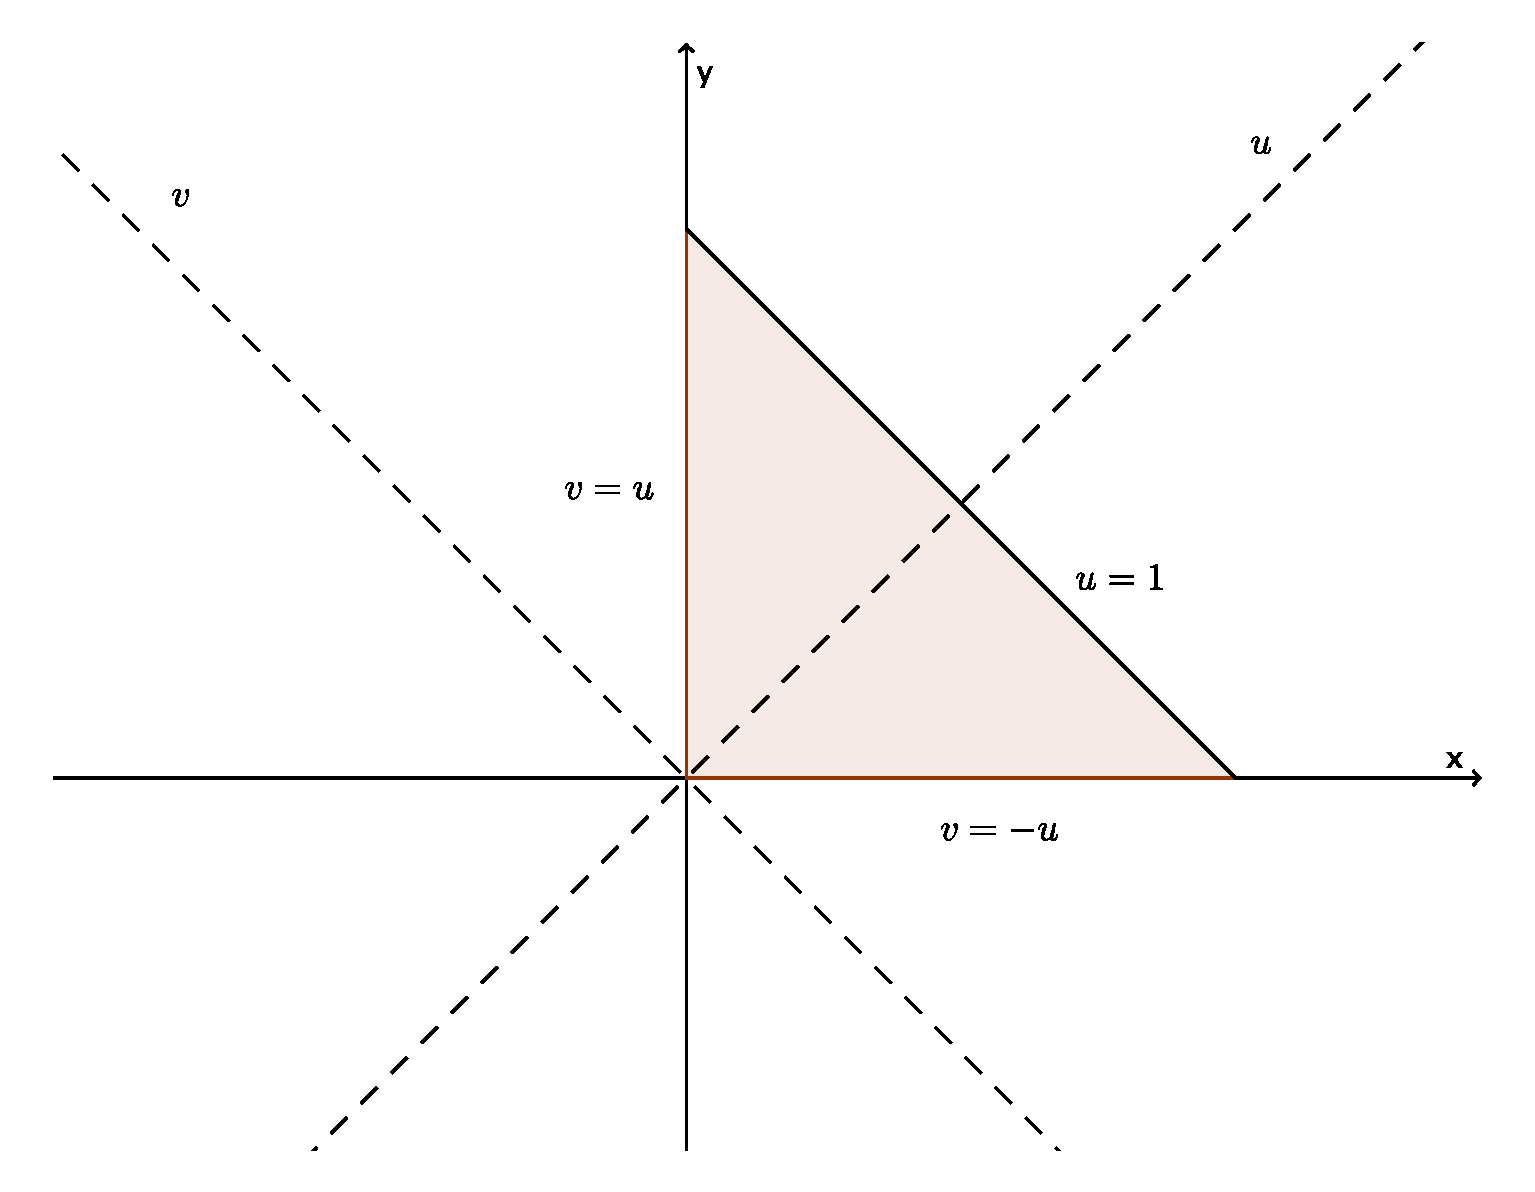
\includegraphics[width=0.5\textwidth]{Q15-bonus}
\end{center}
The Jacobian of the inverse transformation $T^{-1}(x,y) = (x+y,x-y)$ is $J_{T^{-1}}(x,y) = \begin{vmatrix}1&1\\1&-1\end{vmatrix} = -2$, so we have
\[
 \iint_R f(x,y)\,dA = \int_0^1\int_{-u}^u f(u)\lvert -1/2\rvert \,dv\,du = \int_0^1 uf(u)\,du,
\]
as required.

\pagebreak

Additional practice problems:

\begin{enumerate}
\item Let $D$ be the region in the first quadrant bounded by the curves $y=x$, $y=2x$, $xy=1$, and $xy=2$.
\begin{enumerate}
\item Sketch the region, carefully noting all points of intersection of these curves.

\begin{center}
 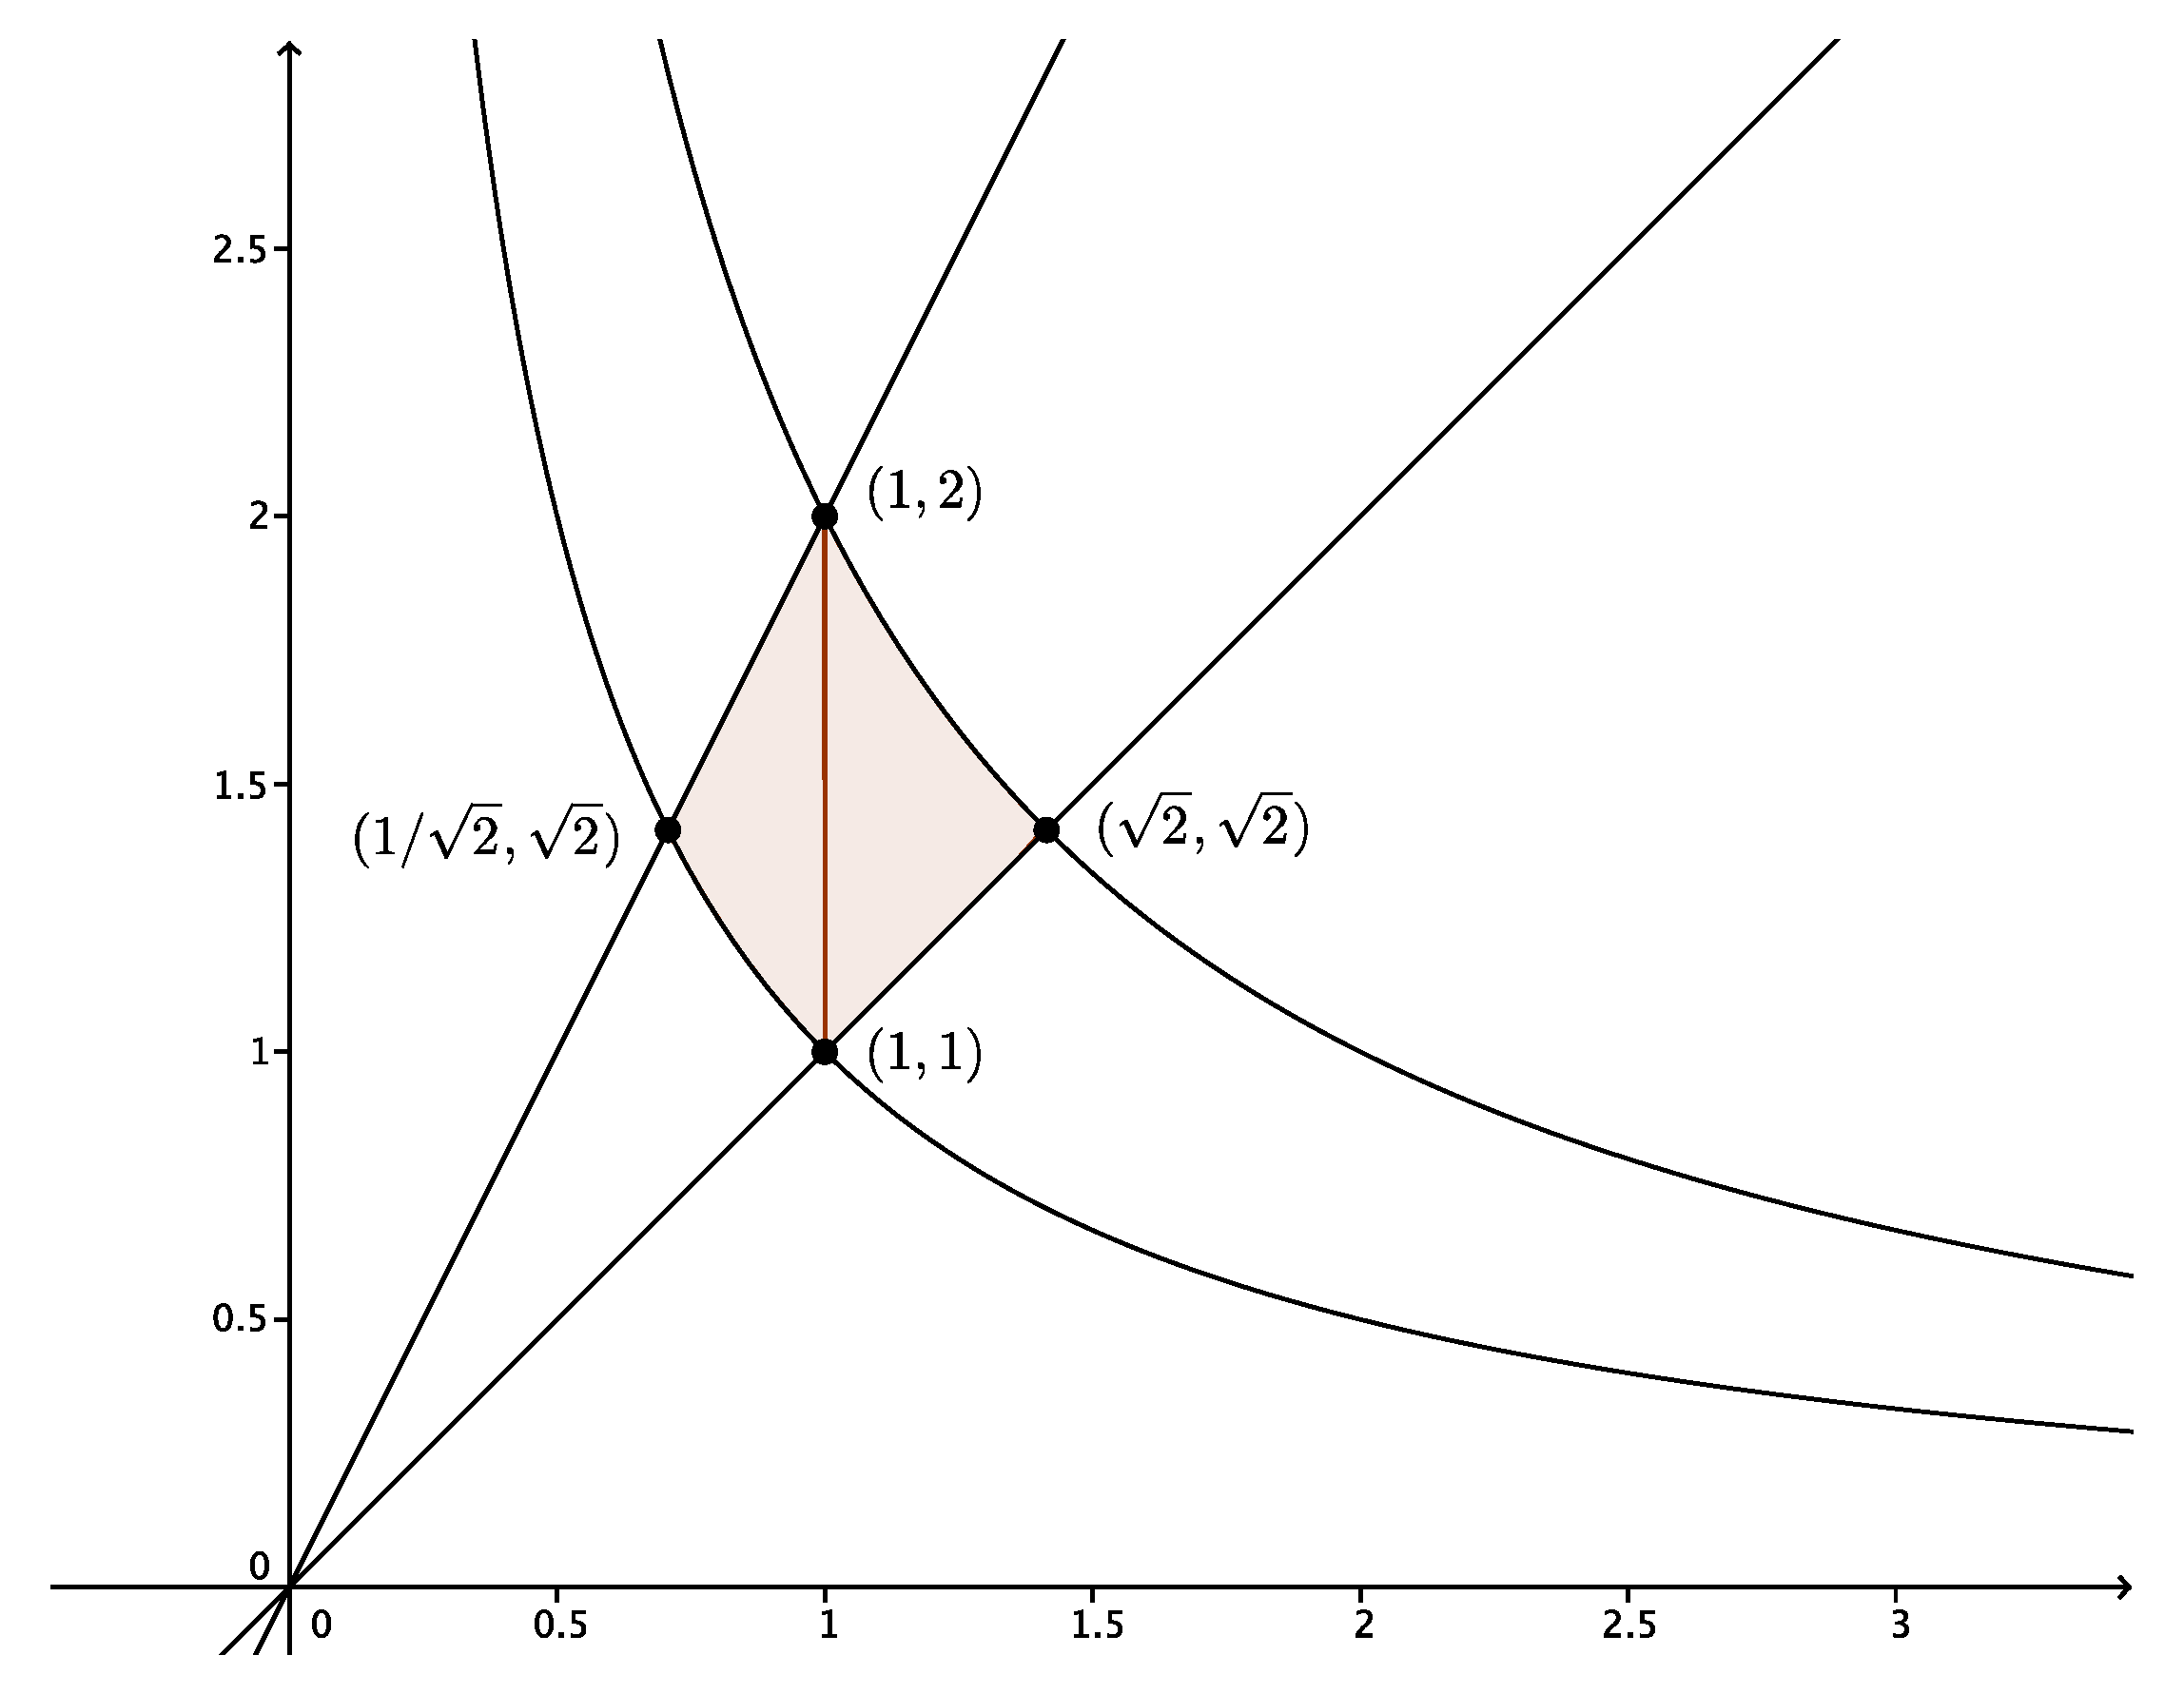
\includegraphics[width=0.7\textwidth]{Q15-extra1}
\end{center}

\item Determine a change of variables that transforms a rectangle in the $(u,v)$-plane into the region $D$.

\bigskip

We can describe the boundary of our region in terms of the level curves $y/x=1$, $y/x=2$, $xy=1$, and $xy=2$. Setting $u=y/x$ and $v=xy$, we have $1\leq u\leq 2$ and $1\leq v\leq 2$. So far we've described the inverse transformation $T^{-1}(x,y) = (y/x, xy)$. To get the desired transformation, we solve for $x$ and $y$ in terms of $u$ and $v$. From $u=y/x$ we have $y=ux$, so $v=xy = x^2u$. This gives us $x^2=v/u$, and for the first quadrant, we take the positive square root, giving us $x=\sqrt{v/u} = u^{-1/2}v^{1/2}$. We then have $y=ux = u^{1/2}v^{1/2}$, so the transformation
\[
 T(u,v) = (u^{-1/2}v^{1/2},u^{1/2}v^{1/2})
\]
transforms the rectangle $[1,2]\times [1,2]$ into the desired region.

\item Use this change of variables to evaluate the integral $\di \iint_D\left(\frac{(x-y)^2}{x^2}-1\right)\,dA$.

First, we note that $\dfrac{(x-y)^2}{x^2}-1 = \dfrac{x^2-2xy+y^2}{x^2}-1 = 1-2\dfrac{y}{x}+\dfrac{y^2}{x^2}-1 = u^2-2u$. Next, we compute
\[
 J_T(u,v) = \det\begin{bmatrix}x_u&x_v\\y_u&y_v\end{bmatrix} = \det\begin{bmatrix} -\frac{1}{2}u^{-3/2}v^{1/2}& \frac{1}{2}u^{-1/2}v^{-1/2}\\ \frac{1}{2}u^{-1/2}v^{1/2}& \frac{1}{2}u^{1/2}v^{-1/2}\end{bmatrix} = -\frac{1}{2u}.
\]
(As an aside, note that $J_{T^{-1}}(x,y) = \begin{vmatrix} -y/x^2 & 1/x\\y&x\end{vmatrix} = -2\dfrac{y}{x} = -2u$, so again we see the reciprocal relationship bewteen the two Jacobians.) Putting everything together, we have
\[
 \iint_D\left(\frac{(x-y)^2}{x^2}-1\right)\,dA = \int_1^2\int_1^2 (u^2-2u)\left\lvert\frac{-1}{2u}\right\lvert\,du\,dv = -\frac{1}{4}.
\]

\end{enumerate}
\item Repeat the problem above, if $D$ is bounded by the curves $y=x^2$, $y=2x^2$, $x=y^2$, and $x=4y^2$, for the integral $\di \iint_D\left(\frac{x^2}{y^4}+\frac{y^2}{x^4}\right)\,dA$.

\begin{enumerate}
 \item The desired region is the one with the vertices A, B, C, D shown in the sketch below:

\begin{center}
 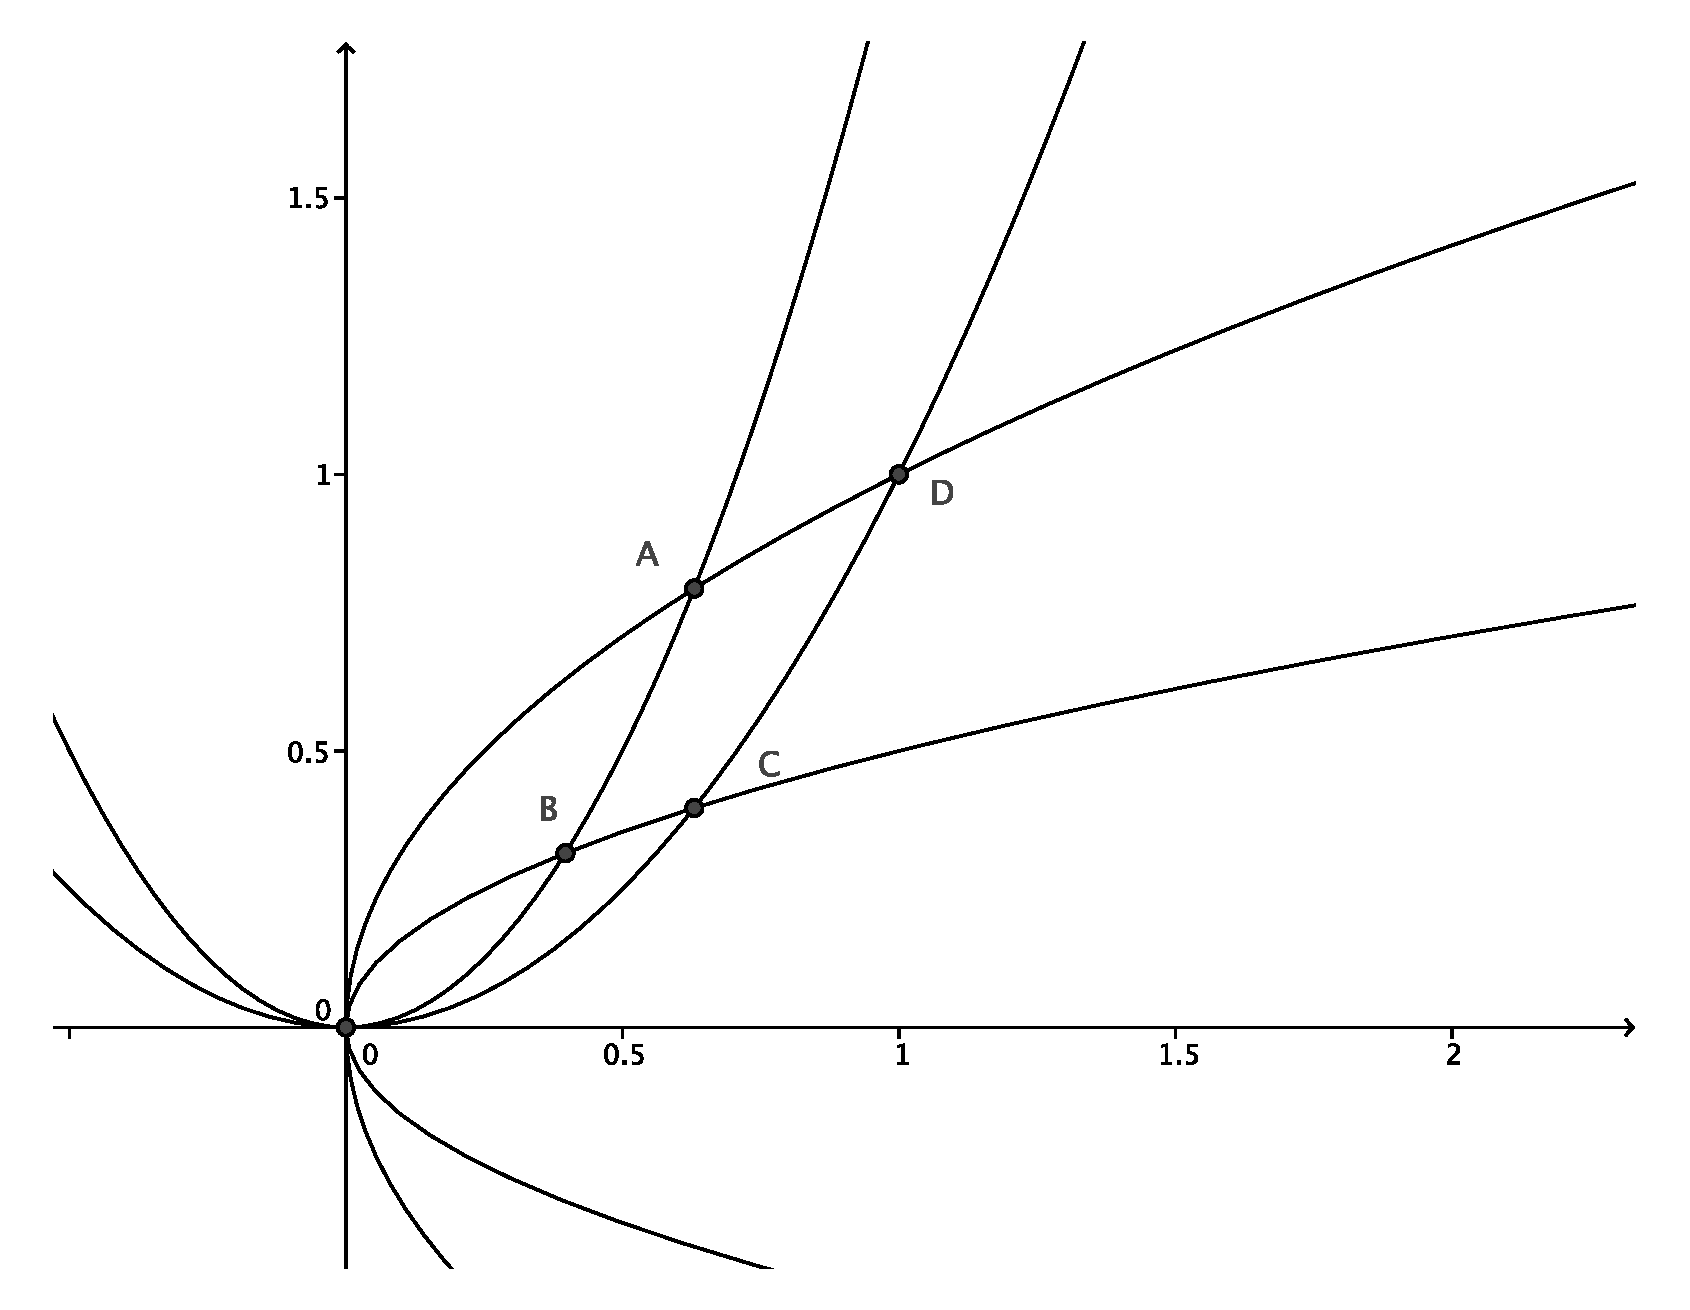
\includegraphics[width=0.7\textwidth]{Q15-extra2}
\end{center}

The points of intersection aren't particularly nice, but we don't really need them to get the change of variables in the next step.

 \item We look to describe the boundaries of our region in terms of families of level curves. In this case we have $1\leq \dfrac{y}{x^2}\leq 2$ and $1\leq \dfrac{x}{y^2}\leq 4$, so we set $u=y/x^2$ and $v=x/y^2$, which defines our inverse transformation $T^{-1}(x,y) = (y/x^2, x/y^2)$. Since $x,y>0$ for our region, we can solve for $x$ and $y$ in terms of $u$ and $v$, giving us $T(u,v) = (u^{-2/3}v^{-1/3}, u^{-1/3}v^{-2/3})$. This isn't particularly pleasant, but fortunately we won't really need it.

 \item To find $J_T(u,v)$ we first compute
\[
 J_{T^{-1}}(x,y) = \begin{vmatrix} -2y/x^3 & 1/x^2\\ 1/y^2 & -2x/y^3\end{vmatrix} = \frac{3}{x^2y^2}
\]
Note that $uv = \dfrac{1}{xy}$, so $J_T(u,v) = \dfrac{1}{J_{T^{-1}}(x,y)} = \frac{x^2}{y^2}{3} = \frac{1}{3u^2v^2}$. This gives us
\[
 \iint_D\left(\frac{x^2}{y^4}+\frac{y^2}{x^4}\right)\,dA = \int_1^2\int_1^4 (u^2+v^2)\frac{1}{3u^2v^2}\,dv\,du = \frac{1}{3}\int_1^2\int_1^4\left(\frac{1}{u^2}+\frac{1}{v^2}\right)\,du\,dv,
\]
and the evaluation of this integral is left as an exercise.
\end{enumerate}

\item Using an appropriate change of variables, show that the area enclosed by the ellipse $\dfrac{x^2}{a^2}+\dfrac{y^2}{b^2}=1$ is $\pi ab$.

\bigskip

Here there is a choice: let $x=au$ and $y=bv$, so that our ellipse is the image of the circle $u^2+v^2=1$ in the $(u,v)$-plane, or let $x=ar\cos\theta$ and $y=br\sin\theta$, as a generalization of the polar coordinate change of variables. 

If we go with the first option, letting $T(u,v) = (au,bv)$, we can easily compute $J_T(u,v) = ab$. Letting $E$ denote the region in the $(x,y)$-plane bounded by the ellipse, and $D$ the region in the $(u,v)$ plane bounded by the unit circle, we have
\[
 \iint_E \,dx\,dy = \iint_D \lvert J_T(u,v)\rvert \,du\,dv = \iint_D ab\,du\,dv = ab\pi,
\]
since the area of the unit disc is $\pi(1)^2=\pi$.

If we go with the second option, letting $T(r,\theta) = (ar\cos\theta, br\sin\theta)$, we have $J_T(r,\theta) = abr$, and we have $0\leq r\leq 1$, and $0\leq \theta\leq 2\pi$, so
\[
 \iint_E \,dx\,dy = \int_0^{2\pi}\int_0^1 abr \,dr\,d\theta = \pi ab.
\]

\item Evaluate $\iint_D \sqrt{x^2+y^2}\,dA$, if $D$ is bounded by the $y$-axis and the curve $y=\sqrt{4-x^2}$.

\bigskip

We evaluate this integral by switching to polar coordinates. The region $D$ is the portion of the disc $x^2+y^2\leq 4$ above the $y$-axis (quadrants I and II), so we have $0\leq r\leq 2$ and $0\leq \theta\leq \pi$. Since $\sqrt{x^2+y^2}=r$, we have
\[
 \iint_D\sqrt{x^2+y^2}\,dA = \int_0^\pi \int_0^2 r\cdot r\,dr\,d\theta = \frac{8\pi}{3}.
\]



\item Evaluate the following integrals, either by converting to polar coordinates, or by reversing the order of integration:
\begin{enumerate}
\item $\di \int_0^4\int_{\sqrt{x}}^2 \frac{1}{y^3+1}\,dy\,dx$.

\bigskip

The limits of integration describe the Type 1 region that lies above the parabola $y=\sqrt{x}$ and below the line $y=2$, to the right of the $y$-axis. As a Type 2 region, this gives us the inequalities $0\leq x\leq y^2$, for $0\leq y\leq 2$. Thus,
\[
 \int_0^4\int_{\sqrt{x}}^2 \frac{1}{y^3+1}\,dy\,dx = \int_0^2\int_0^{y^2}\frac{1}{y^3+1}\,dx\,dy = \int_0^2\frac{y^2}{y^3+1}\,dy = \frac{\ln 9}{3}.
\]

\item $\di \int_0^1\int_y^{\sqrt{2-y^2}}(x+y)\,dx\,dy$.

\bigskip

The limits of integration describe the part of the disc $x^2+y^2\leq 2$ that lies between the lines $y=0$ and $y=x$, in the first quadrant. The region between these lines corresponds to having $\theta\in [0,\pi/4]$, and being within the disc means $0\leq r\leq \sqrt{2}$, so we have
\[
 \int_0^1\int_y^{\sqrt{2-y^2}}(x+y)\,dx\,dy = \int_0^{\pi/4}\int_0^{\sqrt{2}}(r\cos\theta+r\sin\theta)r\,dr\,d\theta = \frac{2\sqrt{2}}{3}
\]


\item $\di \int_{-1}^1\int_0^{\sqrt{1-x^2}}\sqrt{1-y^2}\,dy\,dx$.

\bigskip

This looks like a candidate for polar coordinates, but while the limits of integration come out nicely ($0\leq r\leq 1$, $0\leq \theta\leq \pi$), the integrand does not: we would have to integrate $r\sqrt{1-r^2\sin^2\theta}$.

However, instead of describing the region using the inequalities $0\leq y\leq \sqrt{1-x^2}$, $-1\leq x\leq 1$, we can instead use the inequalities $-\sqrt{1-y^2}\leq x\leq \sqrt{1-y^2}$, $0\leq y\leq 1$. Reversing the order of integration, we have
\[
 \int_{-1}^1\int_0^{\sqrt{1-x^2}}\sqrt{1-y^2}\,dy\,dx = \int_0^1\int_{-\sqrt{1-y^2}}^{\sqrt{1-y^2}}\sqrt{1-y^2}\,dx\,dy = \int_0^1 2(1-y^2)\,dy = \frac{4}{3}.
\]

\end{enumerate}
\end{enumerate}
\end{document}
 
